\section{\sys{} Overview}
\label{sec:overview}

\begin{figure*}[t]
  \centering
  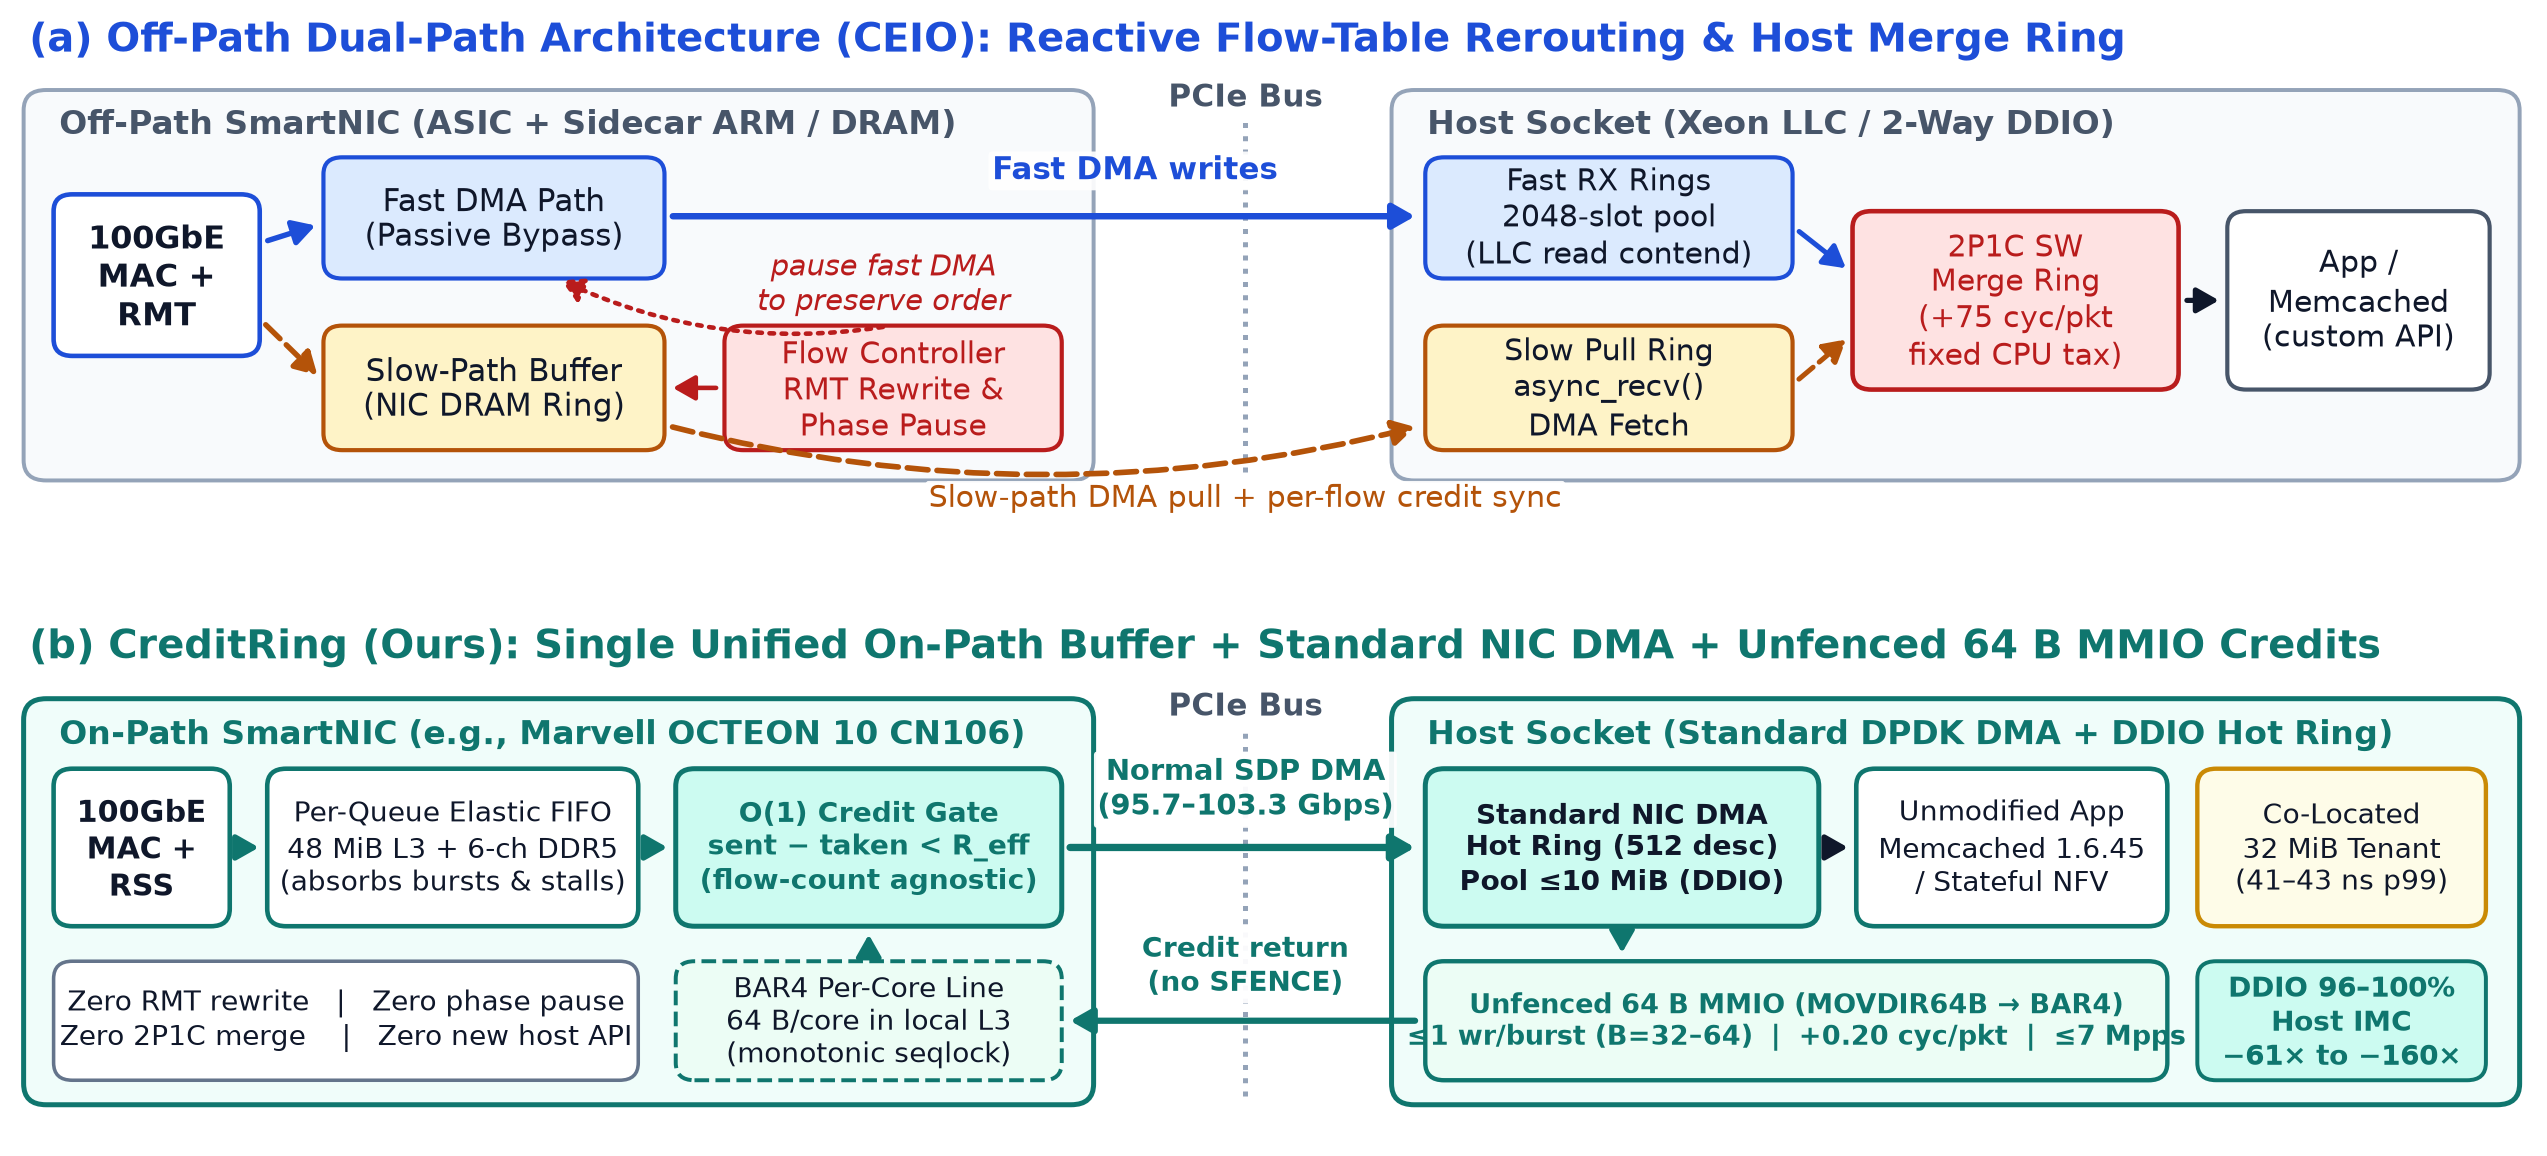
\includegraphics[width=\textwidth]{figures/fig1_architecture.png}
  \caption{Architectural contrast between (a) off-path dual-path caching (\ceio{})
  and (b) \sys{}. Placing an elastic FIFO inline on an on-path SmartNIC while
  preserving standard NIC DMA rings and \texttt{rte\_eth\_rx\_burst()} collapses
  fast delivery and burst buffering into one FIFO gated by unfenced 64\,B MMIO credits.}
  \label{fig:arch}
\end{figure*}

\sys{} assigns burst buffering to an on-path SmartNIC and cache-resident
delivery to standard host DMA rings along a \textbf{single, strictly ordered
FIFO pipeline} (Figure~\ref{fig:arch}(b)). Four design principles eliminate
dual-path complexity while preserving full compatibility with existing host
stacks:

\begin{enumerate}
\item \textbf{Standard NIC DMA data plane and host API.}
  Packets cross PCIe via standard AVX2 \texttt{octeon\_ep} SDP DMA rings with
  no ASIC edits or bespoke transports. Apps receive ordinary \texttt{mbuf}s via
  \texttt{rte\_eth\_rx\_burst()} (no \texttt{async\_recv()} or 2P1C merge ring),
  running unmodified Memcached~1.6.45 with only a $\sim$6-line credit hook and
  16-LoC PMD ring-floor patch (\S\ref{sec:implementation}).
\item \textbf{DDIO-locked rings and pools.}
  Each host queue uses a compact hardware ring ($D=512$ descriptors) gated by a
  tighter logical credit window ($R_{\text{eff}}=128$--$256$) and backed by a
  dedicated compact hot \texttt{mempool} ($\le 10$\,MiB aggregate, yielding
  $\le 7.5$\,MiB actual 1500\,B DMA write footprint). Bounding both in-flight
  count and pool span prevents cold-memory sweeping and dead writebacks.
\item \textbf{Inline $O(1)$ per-queue elastic buffering.}
  On the SmartNIC, every queue $q$ owns an independent FIFO in onboard 48\,MiB
  L3 and 6-channel DDR5. Under normal load, packets stream directly to host
  DMA; whenever bursts or 1--10\,ms host stalls exhaust $q$'s credit budget
  ($\text{submitted}_q - \text{taken}_q \ge R_{\text{eff}}$), excess packets
  queue seamlessly in SmartNIC memory. Tracking two 64-bit counters per queue
  eliminates per-flow tables, RMT rewrites, slow-path rings, phase pauses, and
  flow-churn sensitivity.
\item \textbf{Unfenced 64-byte posted MMIO credit return.}
  Each host core writes batched receive progress (\texttt{taken}, $B=32$--$64$)
  to an exclusive 64-byte BAR4 cache line via a single \emph{unfenced}
  \texttt{MOVDIR64B} per receive burst. The SmartNIC polls this line from local
  coherent L3 ($\sim$10--20\,ns, zero PCIe reads), while aggregate host MMIO
  rate stays within 0.5--7.0\,Mpps---far below the PCIe/mesh interference cliff.
\end{enumerate}
